%\subsection{Traffic Light Controller}
\label{subsec:tlc}
TLC controls an intersection of a busy highway and a little-used farm-way as in Fig. \ref{fig:casestudy}.
Detectors are placed along a farmroad to raise the signal \ti{C} as long as a vehicle is waiting to cross the highway. 
The highway lights remains green as long as no vehicle is detected on the farmroad. 
Otherwise, the highway lights should change from yellow to red, allowing the farmroad lights to become green. 
The farmroad lights stay green only as long as a vehicle is detected on the farmroad and never longer than a set interval to allow the traffic to flow along the highway. 
If no vehicle or timeout expired, the farmroad lights change from green to yellow to red, allowing the highway lights to return to green. 
Even if vehicles are waiting to cross the highway, the highway should remain green for a set interval.




\begin{figure}
	\centering
	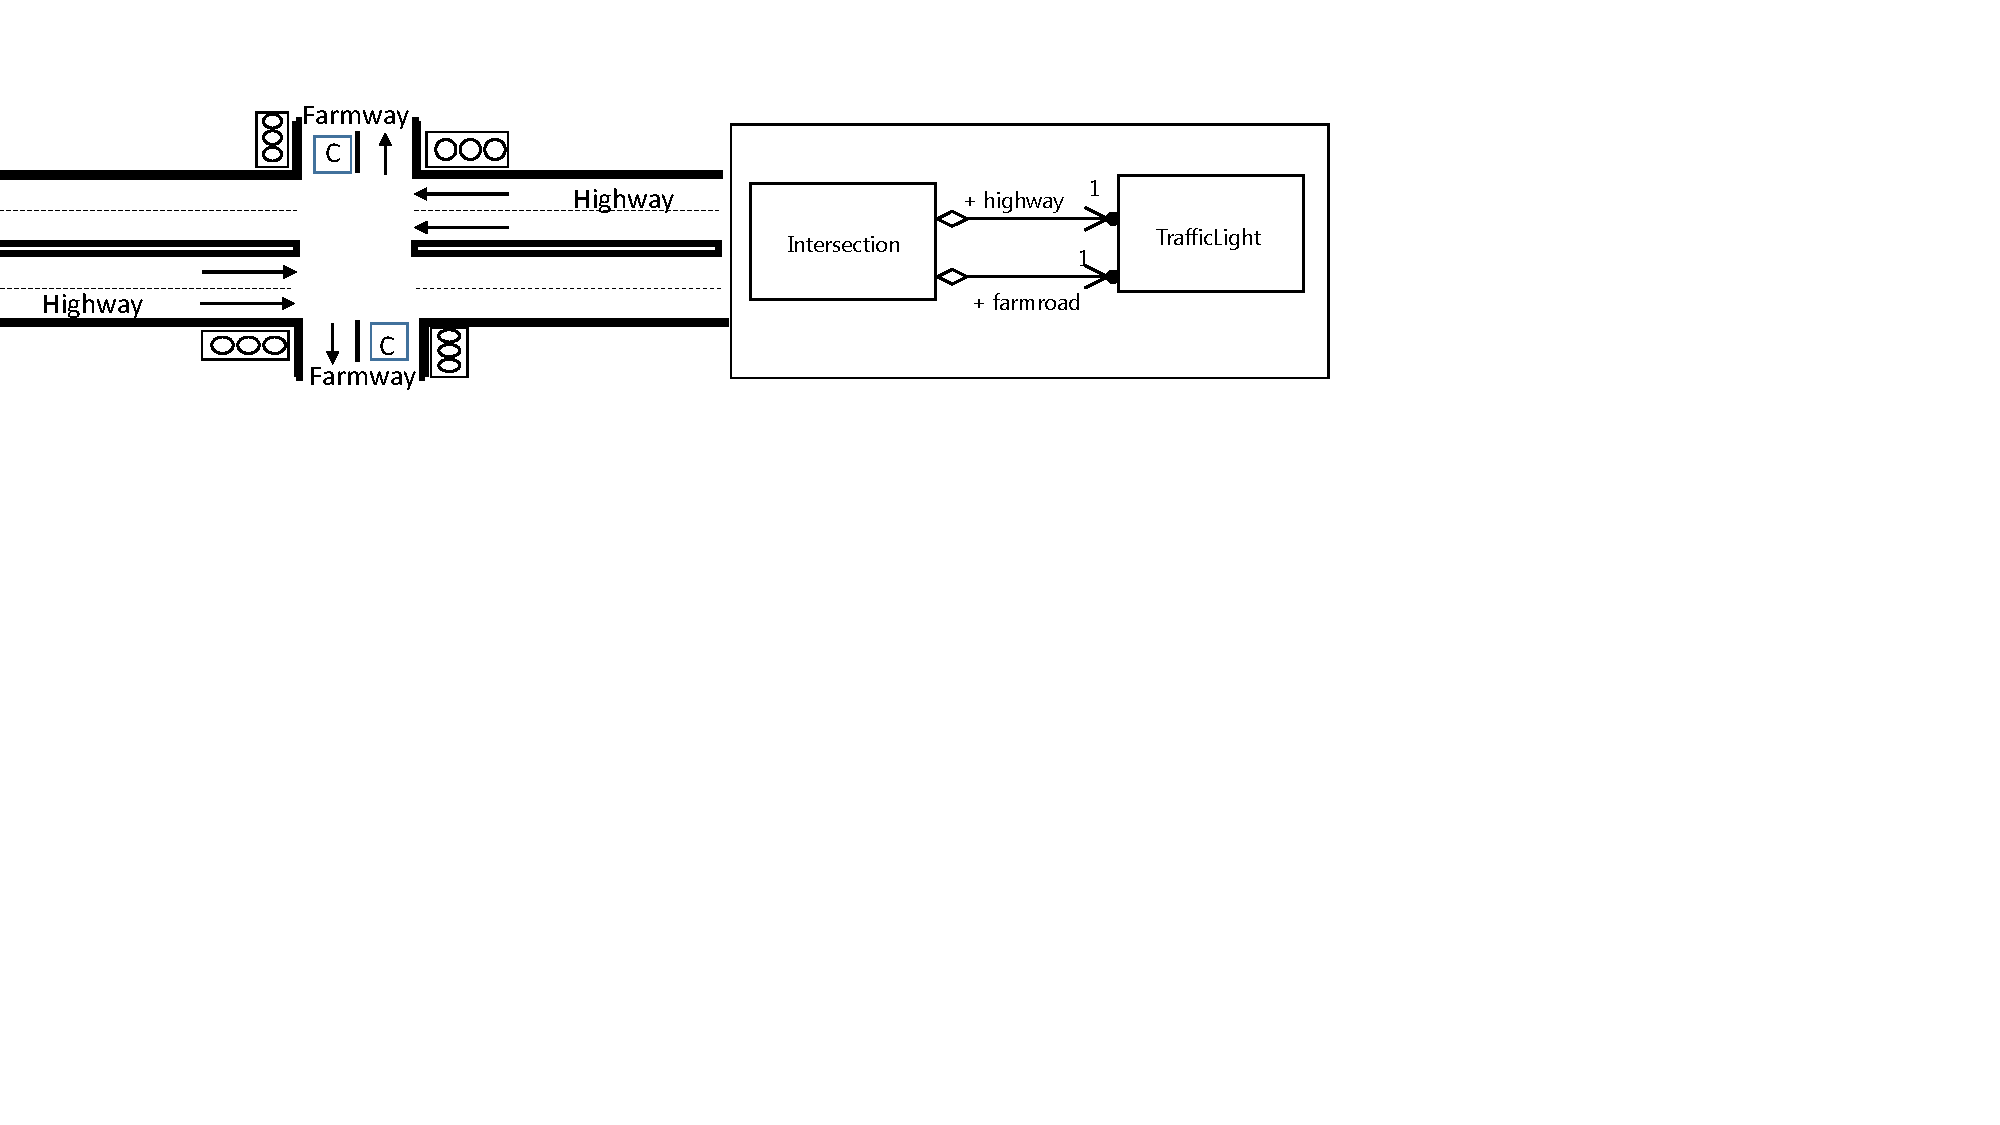
\includegraphics[clip, trim=0.6cm 12.5cm 10.9cm 1.8cm, width=1.0\columnwidth]{figures/casestudy}
	\caption{Traffic Light Controller (left) and its class diagram (right).} 
	\label{fig:casestudy}
\end{figure}


The object-oriented class diagram follows the design in Yasmine \cite{trafficlight}, which is a C++11 state machine framework, and is shown in Fig. \ref{fig:casestudy} (right).
%To emulate the development situation and apply RAOES, a software architect and a programmer participated to the development.
%The class system design is similar to the object-oriented one presented in \cite{trafficlight}.
The behavior of each class is described by a state machine.
%However, the state machine describing the behavior of \ttt{Intersection} in our design is specified by utilizing the deference of events.
The state machines of \ttt{Intersection} and \ttt{TrafficLight} are shown in Fig. \ref{fig:casestudystatemachine} (left and right, respectively).
All of the states of \ttt{IntersectionStateMachine}, except \ttt{FarmwayOpen}, are composite.
The details of \ttt{SwitchingHighwayToFarmroad} and \ttt{SwitchingFarmroadToHighway} are actually shown on the yasmine site \cite{trafficlight}.

\begin{figure}
	\centering
	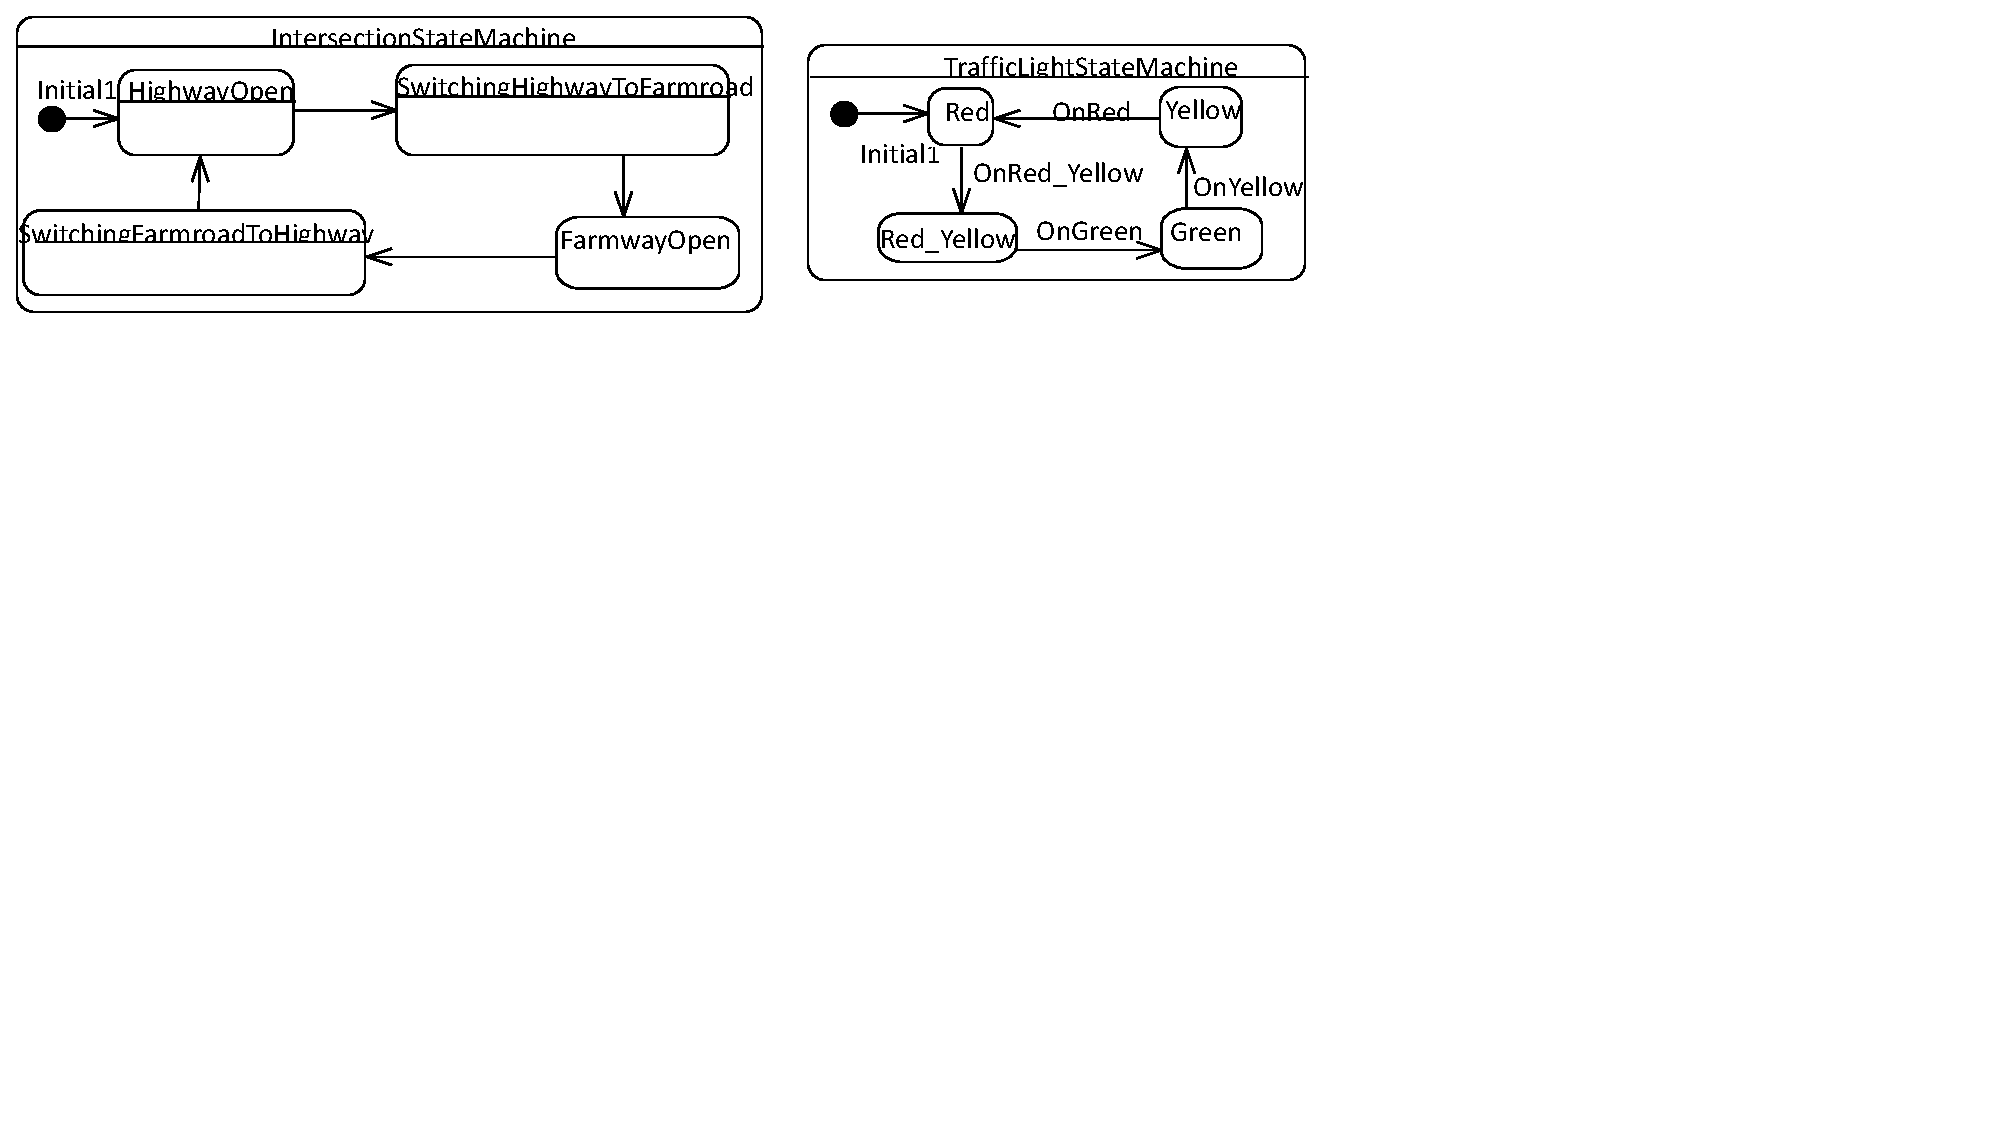
\includegraphics[clip, trim=0.2cm 13.6cm 11.4cm 0.2cm, width=1.0\columnwidth]{figures/casestudystatemachine}
	\caption{State machines for describing the behavior of Intersection (left) and TrafficLight (right)} 
	\label{fig:casestudystatemachine}
\end{figure}


%alternative design for the HighwayOpen composite state
The conditions for switching from the state \ttt{HighwayOpen} to \ttt{SwitchingHighwayToFarmroad} are: (1) a minimum time for the highway open is elapsed; and (2) the sensors emit a signal.

To show the usability and practicality of UML events, two alternative designs can be specified by using time events and change events. 
Fig. \ref{fig:highwayopenalternatives} (a) and (b) show the alternates, respectively.
The first design in \ref{fig:highwayopenalternatives} (a) uses a time event, which triggers the transition from \ttt{WaitingForHighwayMinimum} to \ttt{MinimumTimeElapsed}, and a signal event deferred by the \ttt{WaitingForHighwayMinimum} state. 
When \ttt{HighwayOpen} becomes active, its active sub-state remains \ttt{WaitingForHighwayMinimum} as long as the minimum time.
If a signal C is fired from the detector, a signal event \ttt{DetectorOn} is sent to the state machine.
The event is, however, not immediately processed but delayed by until the active sub-state becomes \ttt{MinimumTimeElapsed} in case the time event is fired.
The signal event is then processed to finish the execution of \ttt{HighwayOpen} and activate the farmway.

The other design utilizes a change event instead of deferred events for switching from \ttt{WaitForPreconditions} to a final state. 
Two flags \ttt{timeFlag} and \ttt{detectFlag} are used.
The \ttt{WaitForPreconditions} state has two internal transitions.
One is triggered by a signal event associated with the signal C and calls a transition effect to update \ttt{detectFlag} to true.
The other one triggered by a time event sets \ttt{timeFlag} to true. 
The expression associated with the change event updates from false to true once two flags \ttt{timeFlag} and \ttt{detectFlag} are set to true. 
The periodic evaluation time is configured as 10ms.
%\ttt{timeFlag} is set by executing the effect \ttt{setTime} of the internal transition of \ttt{WaitForPreconditions} triggered by the \ttt{TE\_MIN} time event. 
%And \ttt{detectFlag} is set by the method \ttt{setDetect} once a \ttt{DetectorOn} event occurs to trigger another internal transition of \ttt{WaitForPreconditions}.
\begin{figure}
	\centering
	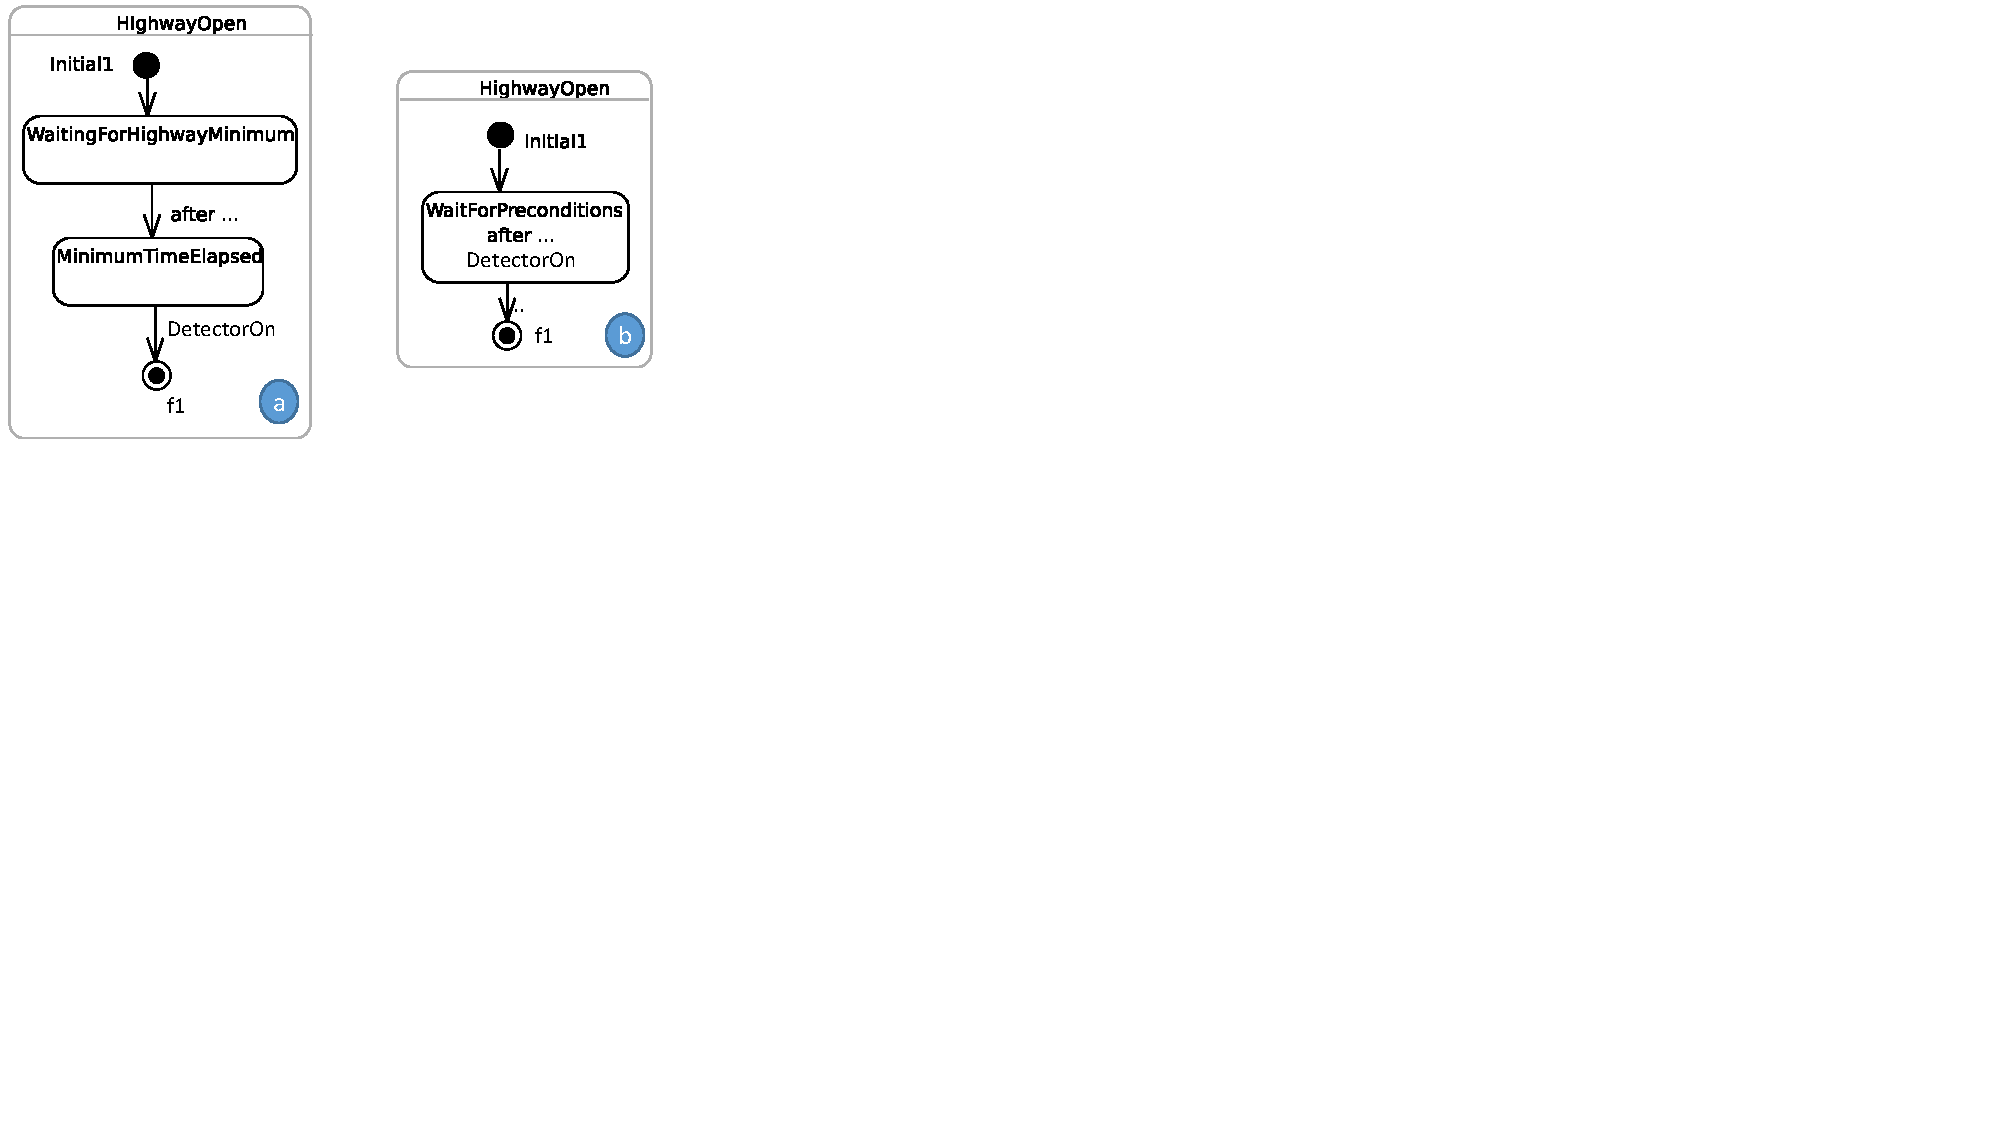
\includegraphics[clip, trim=0.0cm 11.5cm 22.1cm 0cm, width=0.7\columnwidth]{figures/highwayopenalternativesoptimized}
	\caption{Alternative state machine designs for the \ttt{HighwayOpen} state} 
	\label{fig:highwayopenalternatives}
\end{figure}

%The architect creates the USM (using a modeling tool) for \ttt{Intersection} 
%since its behavior is complex and needs graphical tools to represent 
%for better understanding.
%For the programmer, he 
%is more familiar with C++. He 
%develops the low-level behavior and creates the state machine for \ttt{TrafficLight} textually, from scratch.
%These actors worked in parallel and synchronized their assignment after finishing.
%The synchronization is realized by our previously presented process.

For simulation of TLC, we reuse the detector class developed in \cite{trafficlight} to automatically generate \ttt{DetectorOn/DetectorOff} signals. 

The support of UML events (change events and time events) and deferred events does not only provide designers more options to specify but also simplify system behaviors. 
It can also reduce the number of states.
For example, the numbers of sub-states of \ti{HighwayOpen} with the use of deferred events and change events are two and one, respectively, while Yasmine requires three states.   
However, deferred events might make the design more difficult to understand because of its specialized semantics.  

\begin{comment}
\begin{table}[]
	\small
	\centering
	\caption{My caption}
	\label{my-label}
	\begin{tabular}{|l|l|l|l|}
		\hline
		\multirow{2}{*}{Criteria} & \multirow{2}{*}{Yasmine} & \multicolumn{2}{c|}{Our tool}                                                 \\ \cline{3-4} 
		&                          & Normal GCC & \begin{tabular}[c]{@{}l@{}}GCC with \\ optimization\end{tabular} \\ \hline
		LoC                       &                          &            &                                                                  \\ \hline
		Binary size               &                          &            &                                                                  \\ \hline
	\end{tabular}
\end{table}
\end{comment}

%show the state machine and associated code

%show some comparison with the implementation of yasmine: line of code, binary size